\documentclass[border=1pt]{standalone}
\usepackage[dvipsnames]{xcolor}
\usepackage{tikz}                       % Graphen und kommutative Diagramme
\usetikzlibrary{patterns}               % Um schraffierte Formen in der tikzpicture-Umgebung zu zeichnen.

\begin{document}

\newcommand{\ul}{\underline}
\newcommand{\radmult}
{
    \ensuremath{
	\tikz[baseline={([yshift=-1pt]current bounding box.center)}, x=5pt, y=2.5pt, every node/.style={shape=circle, fill=black, inner sep=.8pt}]{
	    \draw[line width=0.9pt] (5, 0) -- (3, 0);
	    \draw[line width=0.9pt] (2, 0) -- (0, 0);
	    \filldraw (3, 0) circle (1pt);
	    \filldraw (2, 0) circle (1pt);
	}
    }
}

\newcommand{\equals}
{
    \ensuremath{
	\tikz[baseline={([yshift=2pt]current bounding box.center)}, x=5pt, y=2.5pt]{
	    \node (0, 0) {$=$};
	}
    }
}


\centering
\begin{minipage}{.55\textwidth}
\centering
\resizebox{!}{5cm}{
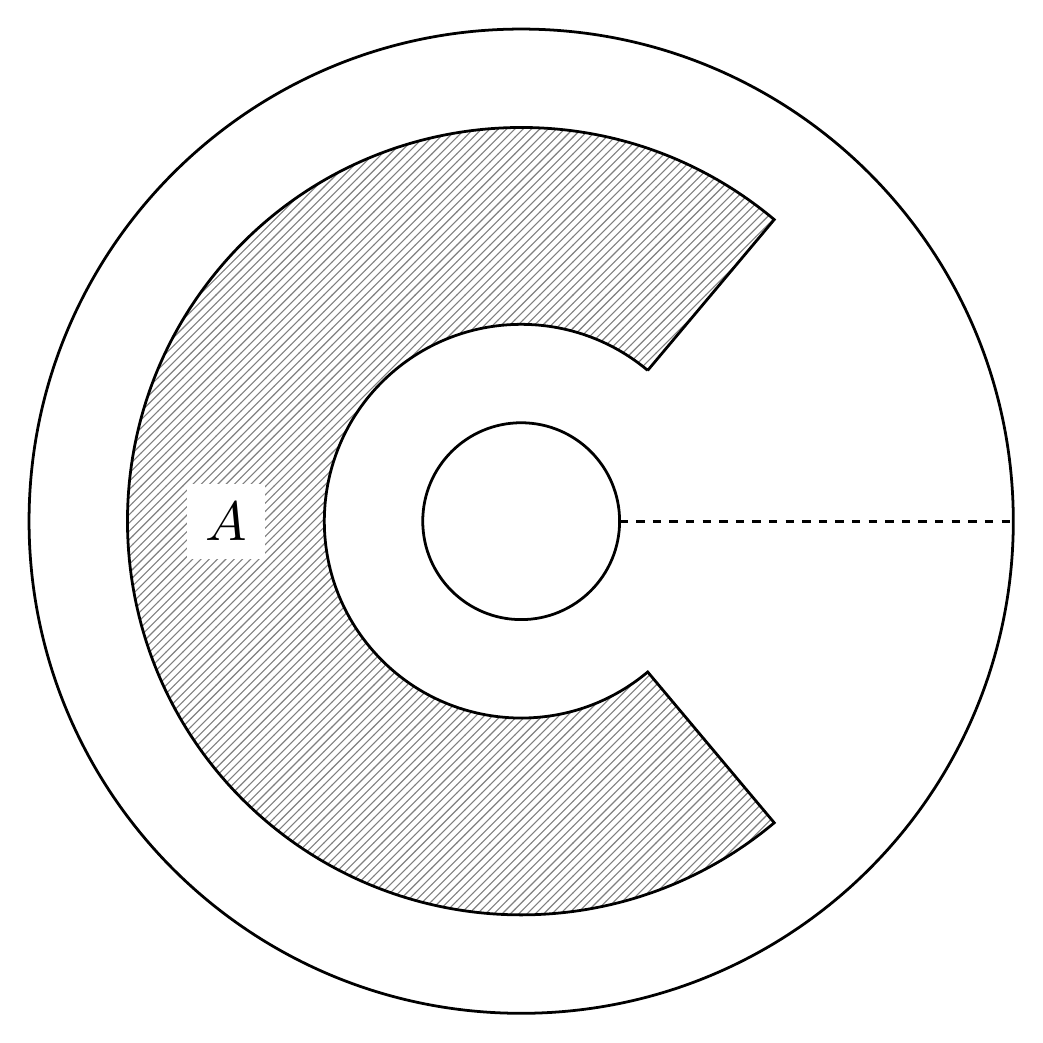
\begin{tikzpicture}[x=1.25cm, y=1.25cm, line width=1pt]
    % draw inner and outer circles
    \draw[color=black] (0, 0) circle (1);
    \draw[color=black] (0, 0) circle (5);
    
    % draw 0 line
    \draw[color=black, dashed] (0 : 1) -- (0 : 5); 
    
    % draw shaded slit box
    \filldraw[pattern=north east lines, pattern color=black!50] 
      (50 : 2) -- (50 : 4) arc [radius = 4, start angle = 50, delta angle = 260] 
	       -- (310 : 2) arc [radius = 2, start angle = 310, delta angle = -260];
    % draw label
    \node[scale = 2, fill = white] at (180 : 3) {$A$};
    
\end{tikzpicture}
}
\end{minipage}

\begin{minipage}{.55\textwidth}
\centering
\resizebox{!}{5cm}{
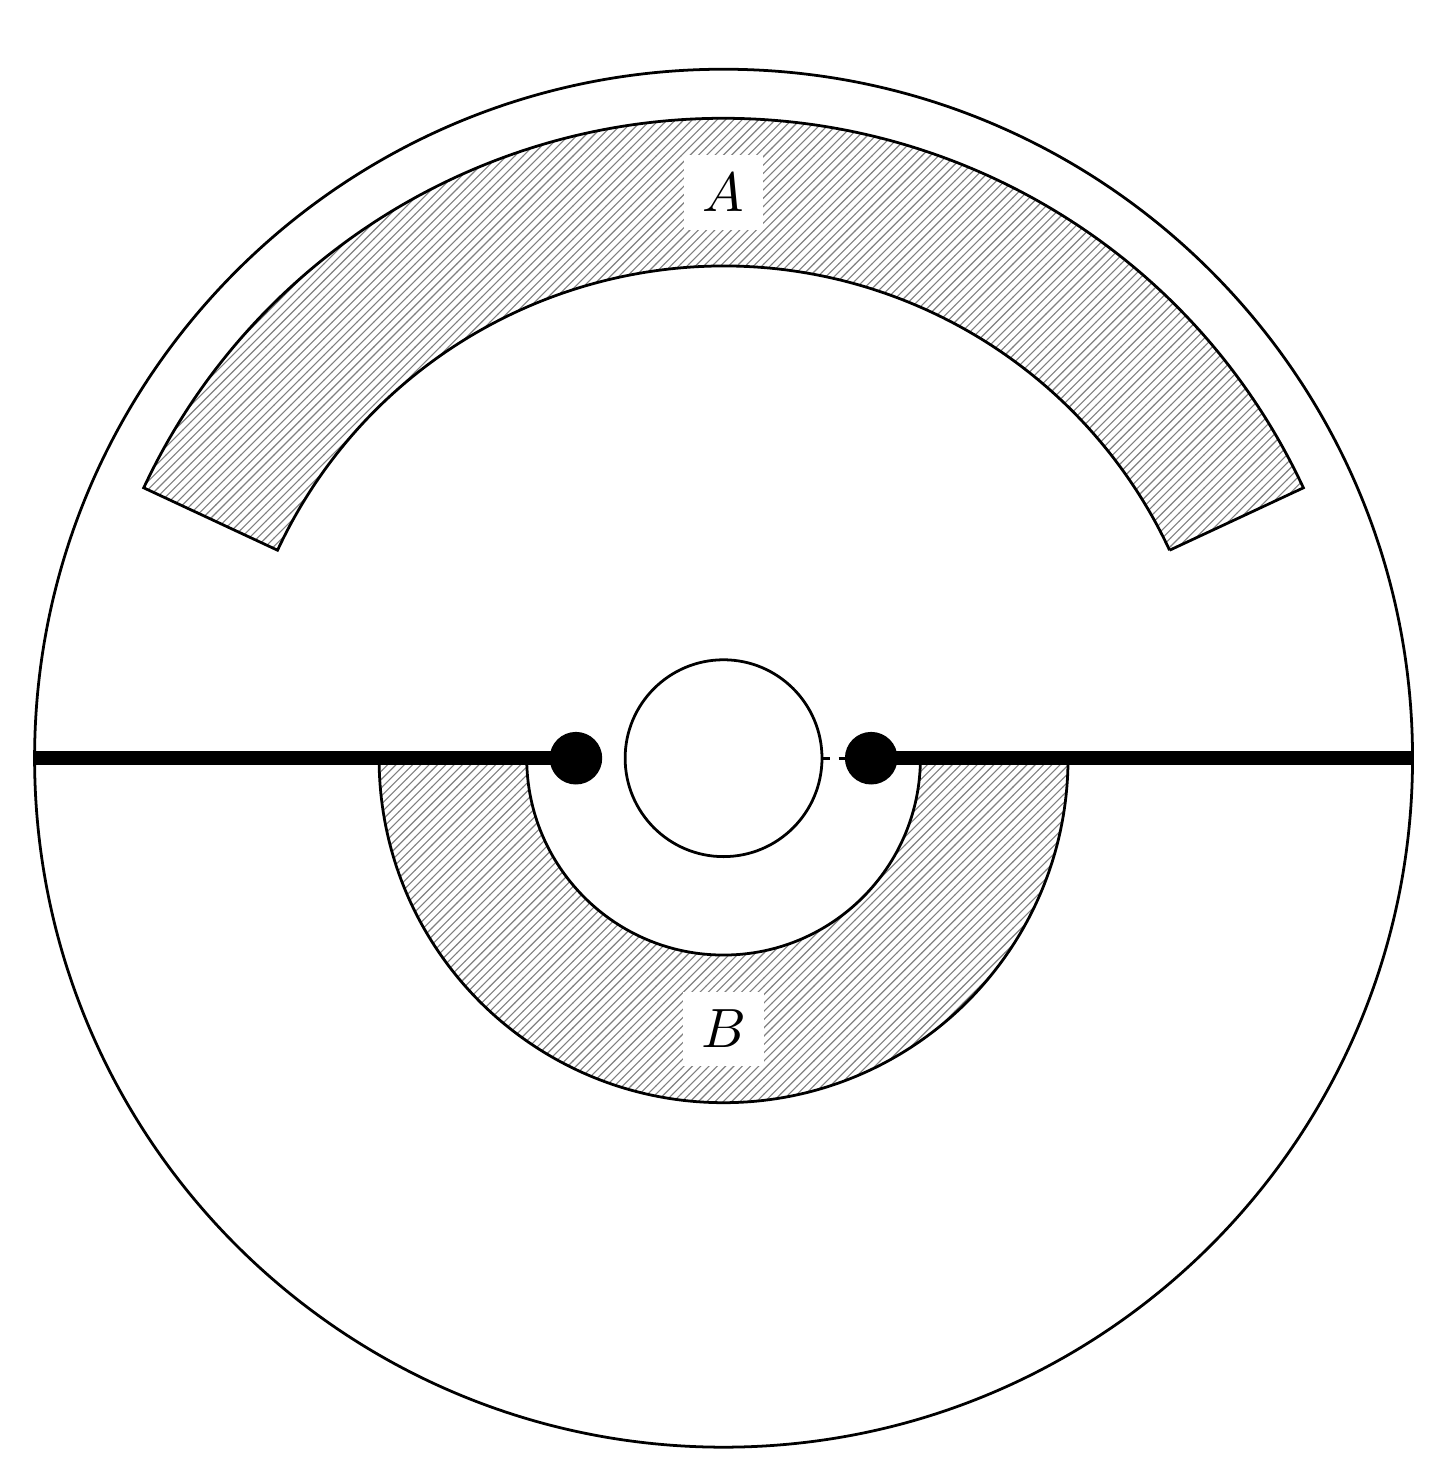
\begin{tikzpicture}[x=1.25cm, y=1.25cm, line width=1pt]
    % draw inner and outer circles
    \draw[color=black] (0, 0) circle (1);
    \draw[color=black] (0, 0) circle (7);
    
    % draw 0 line
    \draw[color=black, dashed] (0 : 1) -- (0 : 7); 
    
    % draw shaded slit box
    \filldraw[pattern=north east lines, pattern color=black!50] 
      (25 : 5) -- (25 : 6.5) arc [radius = 6.5, start angle = 25, delta angle = 130] 
	       -- (155 : 5) arc [radius = 5, start angle = 155, delta angle = -130];
	       
    \filldraw[pattern=north east lines, pattern color=black!50] 
      (0 : 2) -- (0 : 3.5) arc [radius = 3.5, start angle = 0, delta angle = -180] 
	       -- (180 : 2) arc [radius = 2, start angle = 180, delta angle = 180];
    
    % draw label
    \node[scale = 2, fill = white] at (90 : 5.75) {$A$};
    \node[scale = 2, fill = white] at (270 : 2.75) {$B$};
    
    % draw slits
    \draw[color=black, line width=5pt] (1.5, 0) -- (7, 0);
    \filldraw (1.5, 0) circle (9pt);
    \draw[color=black, line width=5pt] (-1.5, 0) -- (-7, 0);
    \filldraw (-1.5, 0) circle (9pt);
    
\end{tikzpicture}
}
\end{minipage}

\end{document}